\documentclass[12pt, a4paper]{article}
\usepackage[margin = 2cm]{geometry}
\usepackage{algorithm}
\usepackage[noend]{algpseudocode}
% Vertical text spacing
\parindent = 0cm \parskip = 0cm
% Section
\usepackage[compact]{titlesec} \titlespacing*{\section}{0pt}{2ex}{2ex}
\titleformat*{\section}{\normalfont\Large\bfseries\color[RGB]{0,0,192}}
\titleformat*{\subsection}{\normalfont\bfseries\color[RGB]{192,0,0}}
% Table spacing
\newcommand\TS{\rule{0pt}{2.6ex}}         % Top strut
\newcommand\BS{\rule[-0.9ex]{0pt}{0pt}}   % Bottom strut
\usepackage{array, multirow}
\newcolumntype{L}[1]{>{\raggedright\TS\BS\arraybackslash}m{#1}}   % Align left
\newcolumntype{C}[1]{>{\centering  \TS\BS\arraybackslash}m{#1}}
\newcolumntype{R}[1]{>{\raggedleft \TS\BS\arraybackslash}m{#1}}   % Align right
% Equations
\usepackage{amsmath, bm, bbold, tikz}

\title{\vspace{-6ex} CO395 Group 57 \vspace{-1ex}}
\author{Dongxiao Huang, Zheng Xun Phang, Yufeng Zhang}
\date{\vspace{-3ex}}

\begin{document}
\maketitle
\pagestyle{plain}
\section*{Implementation}
How do we select the best attribute at each node? For all attributes, we compute the information gain if the dataset is split on that attribute:
\begin{align*}
    \text{Gain(Attribute)} &= \mathcal{I}(p, n) - \left[ \frac{p_0 + n_0}{p + n} \, \mathcal{I}(p_0, n_0) + \frac{p_1 + n_1}{p + n} \, \mathcal{I}(p_1, n_1) \right] \\[0.5ex]
    p_k &= \text{Number of positive examples with (attribute} = k) \\
    n_k &= \text{Number of negative examples with (attribute} = k) \\
    p &= p_0 + p_1 = \text{Number of positive examples before split} \\
    n &= n_0 + n_1 = \text{Number of negative examples before split}
\end{align*}
There are two common ways to measure information.
\begin{flalign*}
    &\text{Entropy:} & \mathcal{I}(p, n) &= - \frac{p}{p+n} \log \frac{p}{p+n} - \frac{n}{p+n} \log \frac{n}{p+n} \qquad \text{if } p, n \neq 0 &\\
    & & \mathcal{I}(p, 0) &= \mathcal{I}(0, n) = 0 &\\[0.5ex]
    &\text{Gini impurity:} & \mathcal{I}(p, n) &= \frac{p}{p+n} \left( 1 - \frac{p}{p+n} \right) + \frac{n}{p+n} \left( 1 - \frac{n}{p+n} \right)
\end{flalign*}
We used entropy since it is stated in the specification, but Gini impurity is faster to compute. Both metrics should give similar results since their graphs have a similar shape:
\begin{center}
\begin{minipage} {0.45 \textwidth}
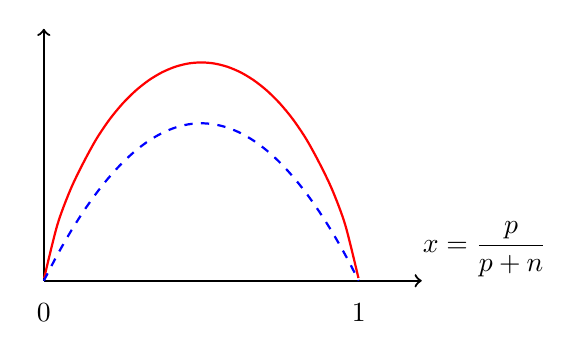
\begin{tikzpicture} [xscale = 4, yscale = 4]
    \draw[->, thick] (0, 0) -- (1.2, 0); 
    \node at (1.4, 0.1) {$\displaystyle x = \frac{p}{p+n}$};
    \draw[->, thick] (0, 0) -- (0, 0.8);
    \newcommand{\gini}[2]    {plot[smooth, domain = #1:#2] (\x, {2 * \x * (1-\x)}) };
    \newcommand{\entropy}[2] {plot[smooth, domain = #1:#2] (\x, {-\x * ln(\x) - (1-\x) * ln(1-\x)}) };
    \draw[thick, red] \entropy{0.001}{0.999};
    \draw[dashed, thick, blue] \gini{0}{1};
    \node at (0, -0.1) {0};
    \node at (1, -0.1) {1};
\end{tikzpicture}
\end{minipage}
\begin{minipage} [b] {0.4 \textwidth}
    {\color{red} Entropy: $-x \log x - (1-x) \log (1-x)$} \\
    \\
    {\color{blue} Gini: $2x (1-x)$}
\end{minipage}
\end{center}
N.B. The \textit{height} of those graphs is irrelevant because minimizing a function is equivalent to minimizing any positive multiple of that function. What matters is their \textit{shape}.\par
\bigskip
The decision tree algorithm is given in the specification, so it's unnecessary to repeat it here. We try to use NumPy functions instead of Python loops for performance since the former run on vectorized C code.\par
\bigskip
To evaluate our decision tree, we performed $K$-fold cross validation as follows:
\begin{enumerate}
    \item Shuffle the dataset and split it into $K = 10$ parts
    \item For each $k \in \{1, \dotsm, K\}$ we train the decision tree on the dataset \textit{excluding} part $k$ and then test the decision tree on part $k$. During testing, we aggregate the predictions from 6 trees (see Ambiguity Question) and increment the relevant cells in the confusion matrix.
\end{enumerate}

\section*{Evaluation}
Each cell of the confusion matrix is a total, not an average, over all folds of cross validation. There were $n = 1000$ test examples in total.\par
\bigskip
\textbf{Warning}: It makes no sense to compute classification rate for each emotion separately. For example, if the actual emotion is Anger then (Fear, Surprise) counts as a true negative for Anger even though it is a misclassification! In other words, if an instance of Fear is misclassified as Surprise, it should not be taken as evidence that our trees are good at detecting Anger.\par
\bigskip
\subsection*{Clean Data}
\begin{center}
\begin{tabular} { C{2.7cm} | C{1.5cm} C{1.5cm} C{1.3cm} C{1.7cm} C{1.5cm} C{1.5cm} }
    \multirow{2}{*}{Actual Class} & \multicolumn{6}{c}{Predicted Class} \\
    & Anger & Disgust & Fear & Happiness & Sadness & Surprise \\ \hline
    Anger     & 97 &  16 &  3 &   4 &  9 &    2 \\
    Disgust   & 19 & 159 &  1 &   7 &  9 &    3 \\
    Fear      &  7 &   4 & 90 &   2 &  3 &   12 \\
    Happiness &  1 &  11 &  2 & 191 &  5 &    5 \\
    Sadness   & 18 &  15 &  5 &   9 & 79 &    6 \\
    Surprise  &  1 &   3 & 11 &   5 &  7 &  179
\end{tabular}
\end{center}
We add up the relevant cells in the confusion matrix above to compute these summary statistics:
\begin{center}
\begin{tabular} { C{2.7cm} | C{1.5cm} C{1.5cm} C{1.3cm} C{1.7cm} C{1.5cm} C{1.5cm} }
    & Anger & Disgust & Fear & Happiness & Sadness & Surprise \\ \hline
    Precision & 0.678 & 0.764 & 0.804 & 0.876 & 0.705 & 0.865 \\
    Recall    & 0.740 & 0.803 & 0.763 & 0.888 & 0.598 & 0.869 \\
    $F_1$ score & 0.708 & 0.783 & 0.783 & 0.882 & 0.648 & 0.867 \\
    --- & 0.920 & 0.912 & 0.950 & 0.949 & 0.914 & 0.945 \\
\end{tabular}
\end{center}
The last row in the table above is the ``classification rate'' of each emotion. As explained earlier, these figures are meaningless. Instead we compute the classification rate of all 6 trees as
\[ \frac{97 + 159 + \dotsm + 179}{1000} = 0.795 \]

\subsection*{Noisy Data}
\begin{center}
\begin{tabular} { C{2.7cm} | C{1.5cm} C{1.5cm} C{1.3cm} C{1.7cm} C{1.5cm} C{1.5cm} }
    \multirow{2}{*}{Actual Class} & \multicolumn{6}{c}{Predicted Class} \\
    & Anger & Disgust & Fear & Happiness & Sadness & Surprise \\ \hline
    Anger     & 30 &  10 &  17 &   8 & 16 &   7 \\
    Disgust   & 13 & 141 &  14 &  11 &  4 &   4 \\
    Fear      & 12 &  15 & 116 &  21 &  8 &  15 \\
    Happiness &  8 &  11 &  12 & 166 &  3 &   8 \\
    Sadness   & 22 &  10 &   5 &   5 & 59 &   9 \\
    Surprise  &  6 &   8 &  15 &  11 &  7 & 173
\end{tabular}
\end{center}
Summary statistics as before:
\begin{center}
\begin{tabular} { C{2.7cm} | C{1.5cm} C{1.5cm} C{1.3cm} C{1.7cm} C{1.5cm} C{1.5cm} }
    & Anger & Disgust & Fear & Happiness & Sadness & Surprise \\ \hline
    Precision & 0.330 & 0.723 & 0.648 & 0.748 & 0.608 & 0.801 \\
    Recall    & 0.341 & 0.754 & 0.620 & 0.798 & 0.536 & 0.786 \\
    $F_1$ score & 0.335 & 0.738 & 0.634 & 0.772 & 0.570 & 0.794 \\
    --- & 0.881 & 0.900 & 0.866 & 0.902 & 0.911 & 0.910 \\
\end{tabular}
\end{center}
\[ \text{Classification rate} = \frac{30 + 141 + \dotsm + 173}{1000} = 0.685 \]
The $F_\alpha$ score by van Rijsbergen (1975) is a harmonic mean of precision $P$ and recall $R$:
\[ \frac{1 + \alpha^2}{F_\alpha} = \frac1P + \frac{\alpha^2}{R} \qquad
   \Rightarrow \qquad F_\alpha = \frac{(1+\alpha^2) PR}{\alpha^2 P + R} \]
which allows us to adjust the weight given to precision or recall. This is useful if, for example, it is essential to detect Anger in an image when it is present. This averaging also enables $F_\alpha$ to deal with imbalanced classes.\par
\bigskip
On clean data, our 6 trees classify the emotions \textit{Disgust}, \textit{Fear}, \textit{Happiness} and \textit{Surprise} with high accuracy ($F_1 > 0.78$) while \textit{Sadness} is harder to detect.\par
\bigskip
On noisy data, our 6 trees classify the emotions \textit{Disgust}, \textit{Happiness} and \textit{Surprise} with high accuracy ($F_1 > 0.73$) while \textit{Anger} and \textit{Sadness} are harder to recognize.\par
\bigskip
We expected emotions to be most frequently misclassified as \textit{Anger} because if none of our 6 trees detect any emotion in an image, then we classify it as \textit{Anger} by default. However, this is not evident from the confusion matrices. In fact, none of our test observations was classified in this manner.\par
\bigskip
The Facial Action Coding System in the specification has more rules that map to \textit{Anger} and \textit{Fear} than to other emotions. This suggests there are more ways for a face to express anger and fear (through action units) than other emotions, so images are likely to be misclassified as such. However, this hypothesis isn't supported by the confusion matrices.\par
\bigskip
We could have created another label ``No emotion'' for images that cannot be classified as any of the 6 emotions. However the specification requires our testTrees(...) function generate predictions in $\{1, \dotsm, 6\}$.

\section*{Miscellaneous}
\subsection*{Noisy-Clean Datasets Question}
Overall performance:\par
Not surprisingly, the noisy dataset has lower overall performance. Its classification rate is 0.685 compared to 0.795 for clean data.\par
\bigskip
Per emotion performance:\par
The conclusion is the same when we analyse each emotion separately: precision, recall and $F_1$ score are lower for noisy data.\par
\bigskip
Noise degrades the classification accuracy of any machine learning model because it won't be learning the true underlying function that maps features to the target variable. For decision trees, this means taking many wrong branches to fit the noise.\par
\bigskip
Another intuition is that as noise in the data increases, the features that predict each emotion will become random, and so a decision tree will effectively be guessing randomly.\par
\bigskip
Among the 6 emotions, \textit{Anger} is most susceptible to noise because a fair number of noisy test examples will not be classified as having any of the 6 emotions, so it is labelled as \textit{Anger} by default. As a result, its $F_1$ score is 0.335 only.\par
\bigskip
\subsection*{Ambiguity Question}
If no emotion is detected, then we predict \textit{Anger}. But if our 6 trees predict that a given face has more than one emotion, we considered several methods of selecting only one emotion:\par
\bigskip
1. Select the first detected emotion in alphabetical order\par
\bigskip
Examples: If \textit{Fear} and \textit{Surprise} are detected, then we predict \textit{Fear}.\par
\bigskip
Advantage: Easy to implement\par
Disadvantage: This method is arbitrary and will not improve the classification rate\par
\bigskip
2A. Select the emotion that was detected from the shallowest node\par
\bigskip
Example: A face gets a positive result from our \textit{Anger} and \textit{Fear} trees. In the \textit{Anger} tree, the face belongs to a node that is 3 levels deep. In the \textit{Fear} tree, it belongs to a node that is 6 levels deep. We classify this face as \textit{Anger}.\par
\bigskip
Advantage: This is more principled than method 1 and simpler than method 3. It may work well if a shallow tree is sufficient to fit the data, since it ignores deeper but overfitting trees.\par
Disadvantage: It may not perform well if a deep tree is necessary, since it select the shallowest but underfitting tree.\par
\bigskip
2B. Select the emotion that was detected from the deepest node\par
\bigskip
This contrasts with method 2A above.\par
\bigskip
3. Toggle each action unit in turn and take a majority vote\par
\bigskip
This is our preferred method. Its rationale is: adding or removing an action unit is akin to hiding a part of a face, which does not change its underlying emotion. Of course, if we change too many action units from present to absent or vice versa, then we cannot expect our trees to classify the face correctly. Hence, we only toggle one action unit at a time.\par
\bigskip
Example: A face has action units 3, 7, 12. It gets a positive result from our \textit{Anger} and \textit{Fear} trees. We disable each action unit in turn and test it on our 6 trees as follows.\par
\begin{center}
\begin{tabular} { C{3cm} C{3cm} }
    Action Units & Result \\ \hline
    7, 12 & Fear, Sadness \\
    3, 12 & (none)        \\
    3, 7  & Disgust, Fear \\
\end{tabular}
\end{center}
Since \textit{Fear} is the most frequent result, it will be our prediction.

\begin{algorithm}
\caption{most\_similar(Tree, Features)}\label{euclid}
\begin{algorithmic}[1]
\Function{most\_similar}{T, F}
\For{\texttt{$f \subseteq F$}}
        \State \texttt{toggle $f$}
        \For{\texttt{$e \subseteq emotions$:}}
        \State \texttt{TEST-TREE($F$) for $e$}
        \State \texttt{add score for $e$}
        \EndFor
		\State \texttt{toggle $f$}

\EndFor
\Return scores
\EndFunction
\label{code3}
\end{algorithmic}
\end{algorithm}

Advantage: This method has the best classification rate among the 3. It is robust to noise.\par
Disadvantage: Test time increases with the number of action units.\par
\bigskip
The classification rates for the methods above are computed using 10-fold cross validation. The results are presented below.
\begin{center}
\begin{tabular} { C{4cm} | C{1.5cm} C{1.5cm} C{1.5cm} C{1.5cm} }
    Classification Rate & Plan 1 & Plan 2A & Plan 2B & Plan 3 \\ \hline
    Clean Data & 0.726 & 0.719 & 0.715 & 0.795 \\
    Noisy Data & 0.594 & 0.610 & 0.595 & 0.685  \\
\end{tabular}
\label{table}
\end{center}

\subsection*{Pruning Question}
The function $pruning\_example(x, y)$ takes two inputs: $x$ is an $n \times p$ matrix of features and $y$ is a $n$-dimensional vector of target variables.\par
\bigskip
It builds a classification tree and prunes it to various sizes (as measured by number of leaves instead of depth). It computes the classification cost for each tree size. Finally it returns a plot of classification cost against tree size, which also marks the smallest tree size whose cost is within 1 standard error of the minimum cost.\par
\bigskip
The two curves in the plot correspond to two methods of computing classification costs.
\begin{itemize}
    \item Resubstitution: Tests a tree using the same data that was used to fit the tree (i.e. computes in-sample error)
    \item 10-fold cross validation: See our explanation in the Implementation section earlier. Validation error is an out-of-sample error if we don't use it to tune a hyperparameter such as maximum depth, otherwise it's only an estimate of out-of-sample error.
\end{itemize}

\begin{figure} [hp!]
\centering
\includegraphics[width = 0.9 \textwidth] {pruneAnalysis/clean_data_analyse.png}
\caption{Clean Data}
\label{clean}
\end{figure}

\begin{figure} [hp!]
\centering
\includegraphics[width = 0.9 \textwidth] {pruneAnalysis/noisy_data_analyse.png}
\caption{Noisy Data}
\label{noisy}
\end{figure}

In figures \ref{clean} and \ref{noisy}, we find that classification costs have similar behaviour on both clean and noisy data: Resubstitution error keeps falling as the tree gets larger, while validation error falls initially and then rises.\par
\bigskip
This is expected because a deeper tree will always fit a dataset better than a shallower tree. However if a tree is too deep, it will overfit the training data but fail to generalize to unseen data, which is manifested in the increasing validation error.\par
\bigskip
Differences between clean and noisy data:
\begin{itemize}
    \item For a fixed tree size, resubstitution and validation errors are higher on noisy data than clean data, since noise by definition makes it harder for a tree to fit the data.
    \item For the same reason, noisy data require more branches, and hence more leaves, to classify all training examples. It took about 275 vs 200 leaves to achieve zero in-sample error.
    \item The gap between resubstitution and validation errors rises faster for noisy data than clean data, which shows that overfitting is more severe when the data have noise.
\end{itemize}
Optimal tree size for clean data is about 22 leaves while that for noisy data is 25 leaves.\par

\newpage

\section*{Tree Diagrams}
Figure \ref{firstTree} to \ref{lastTree} are the trees trained on the entire clean dataset (1004 examples).

\begin{figure}[h!]
\centering
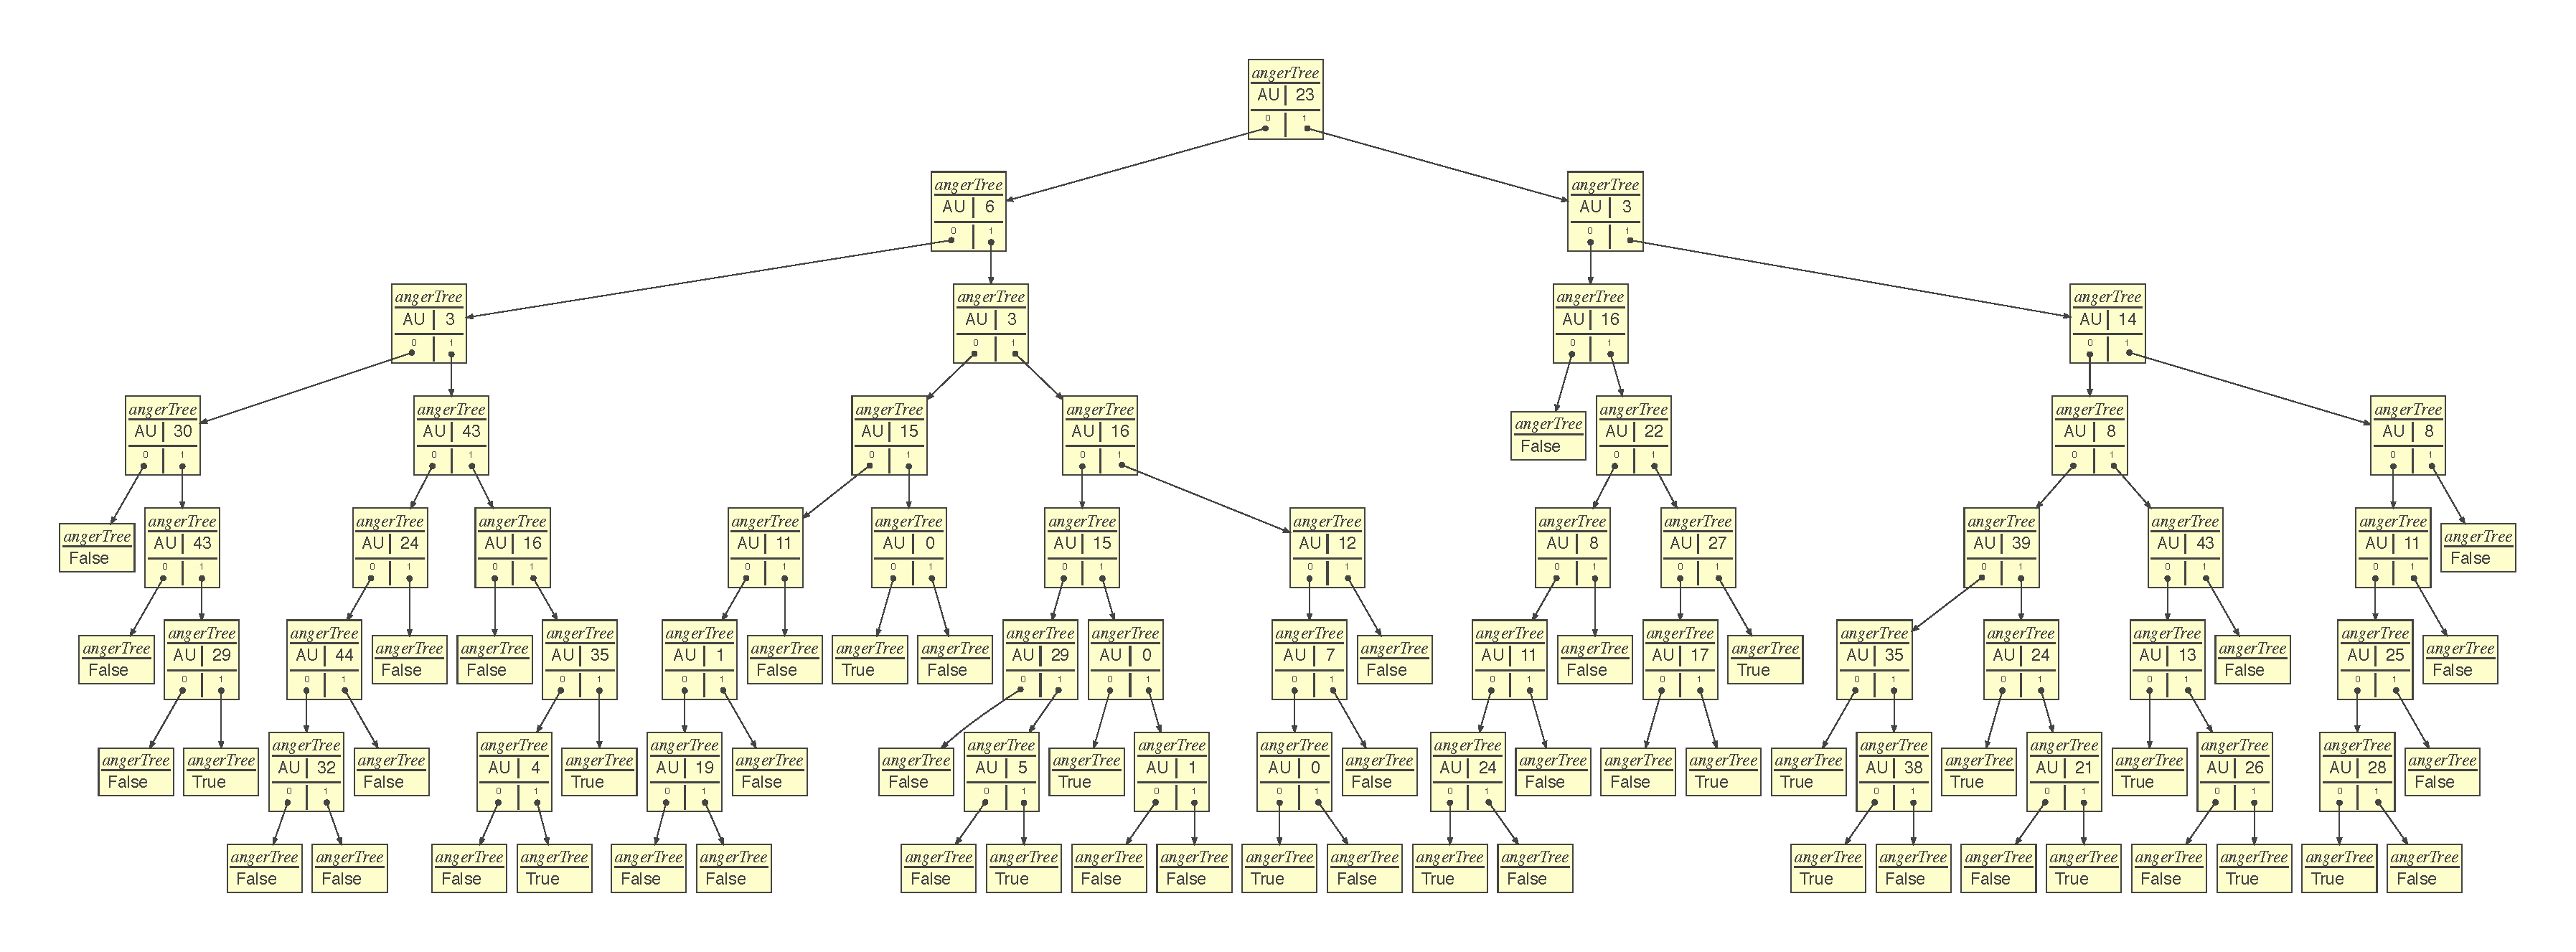
\includegraphics[width=\textwidth]{treePics/angerTree.pdf}
\caption{Anger Tree}
\label{firstTree}
\end{figure}
\begin{figure}[h!]
\centering
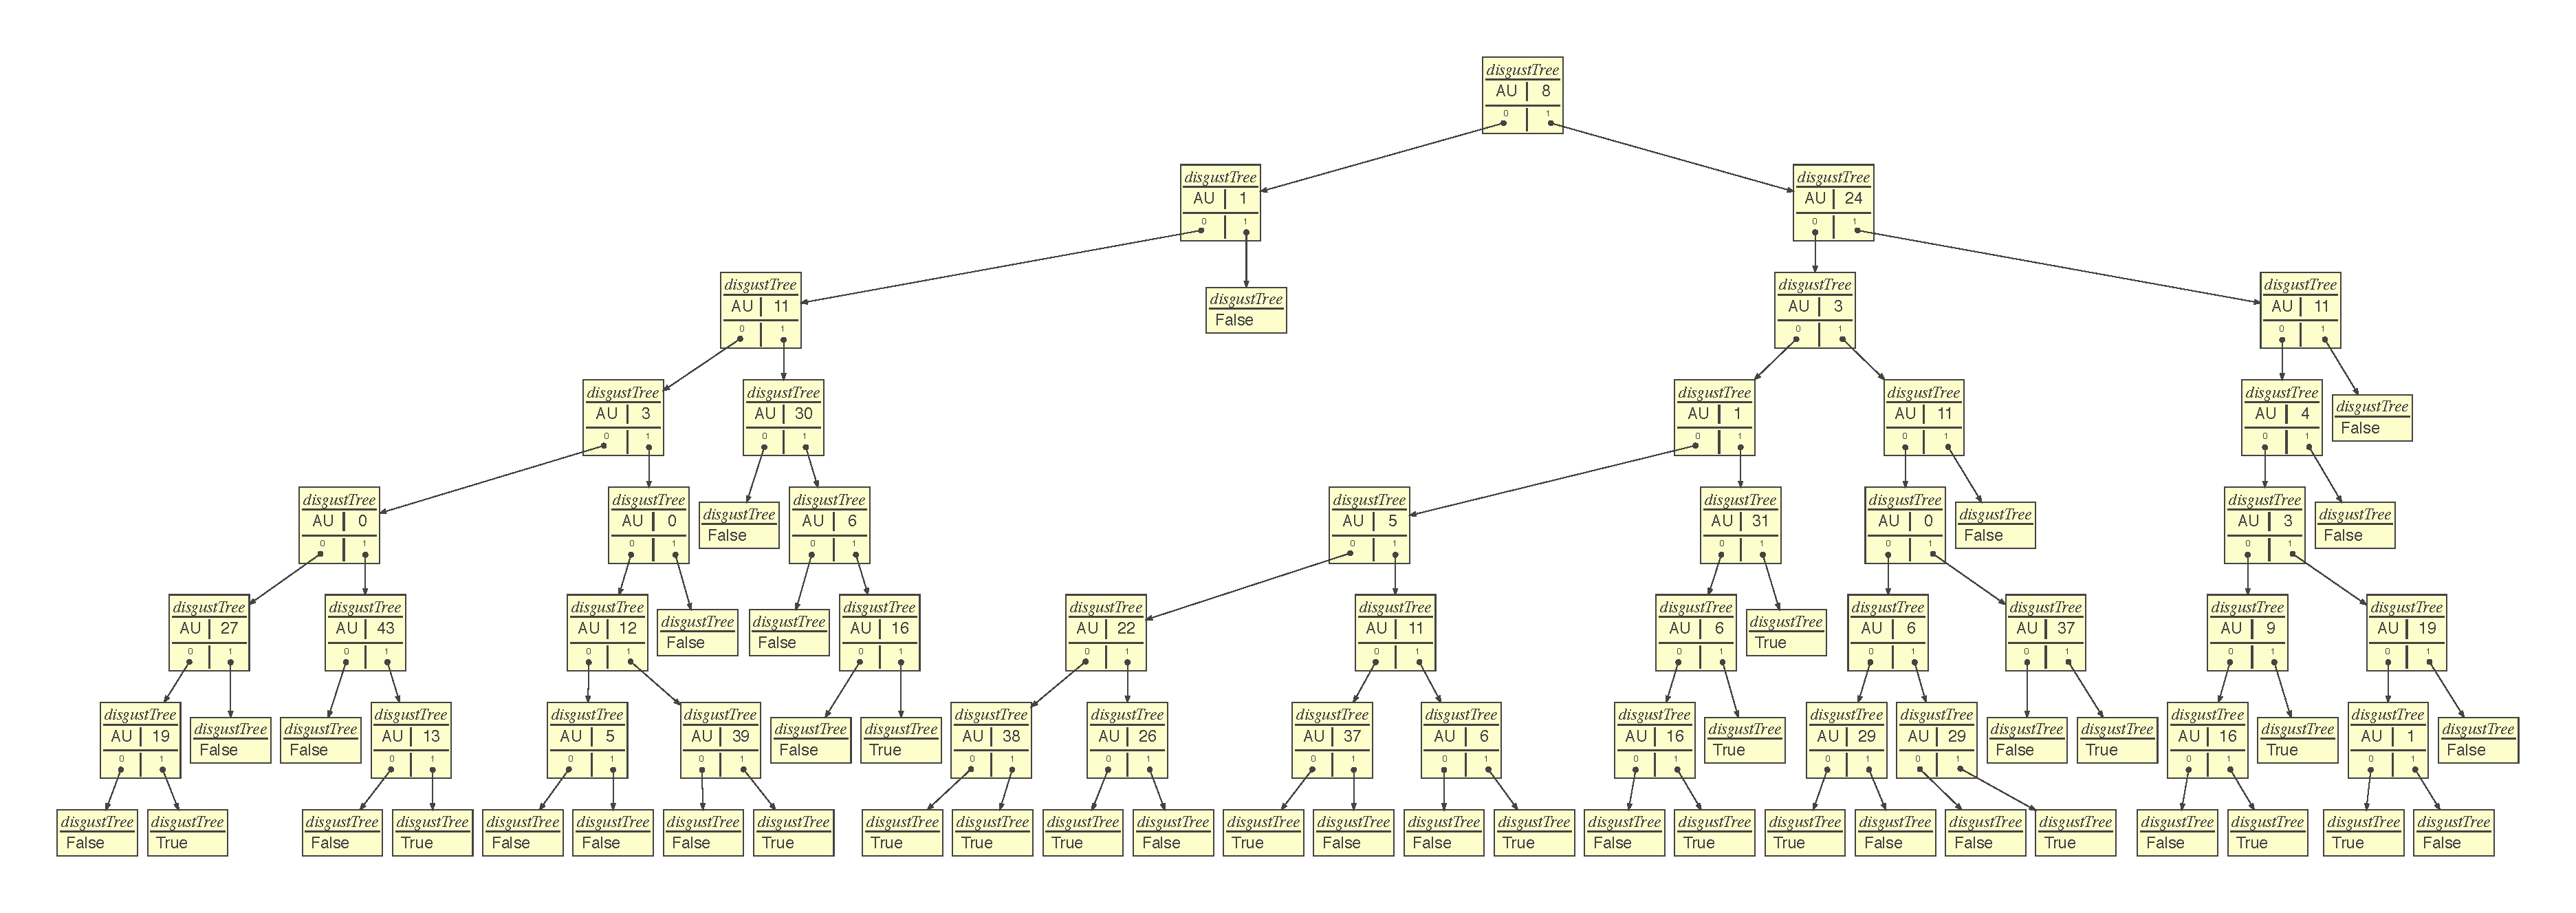
\includegraphics[width=\textwidth]{treePics/disgustTree.pdf}
\caption{Disgust Tree}
\end{figure}
\begin{figure}[h!]
\centering
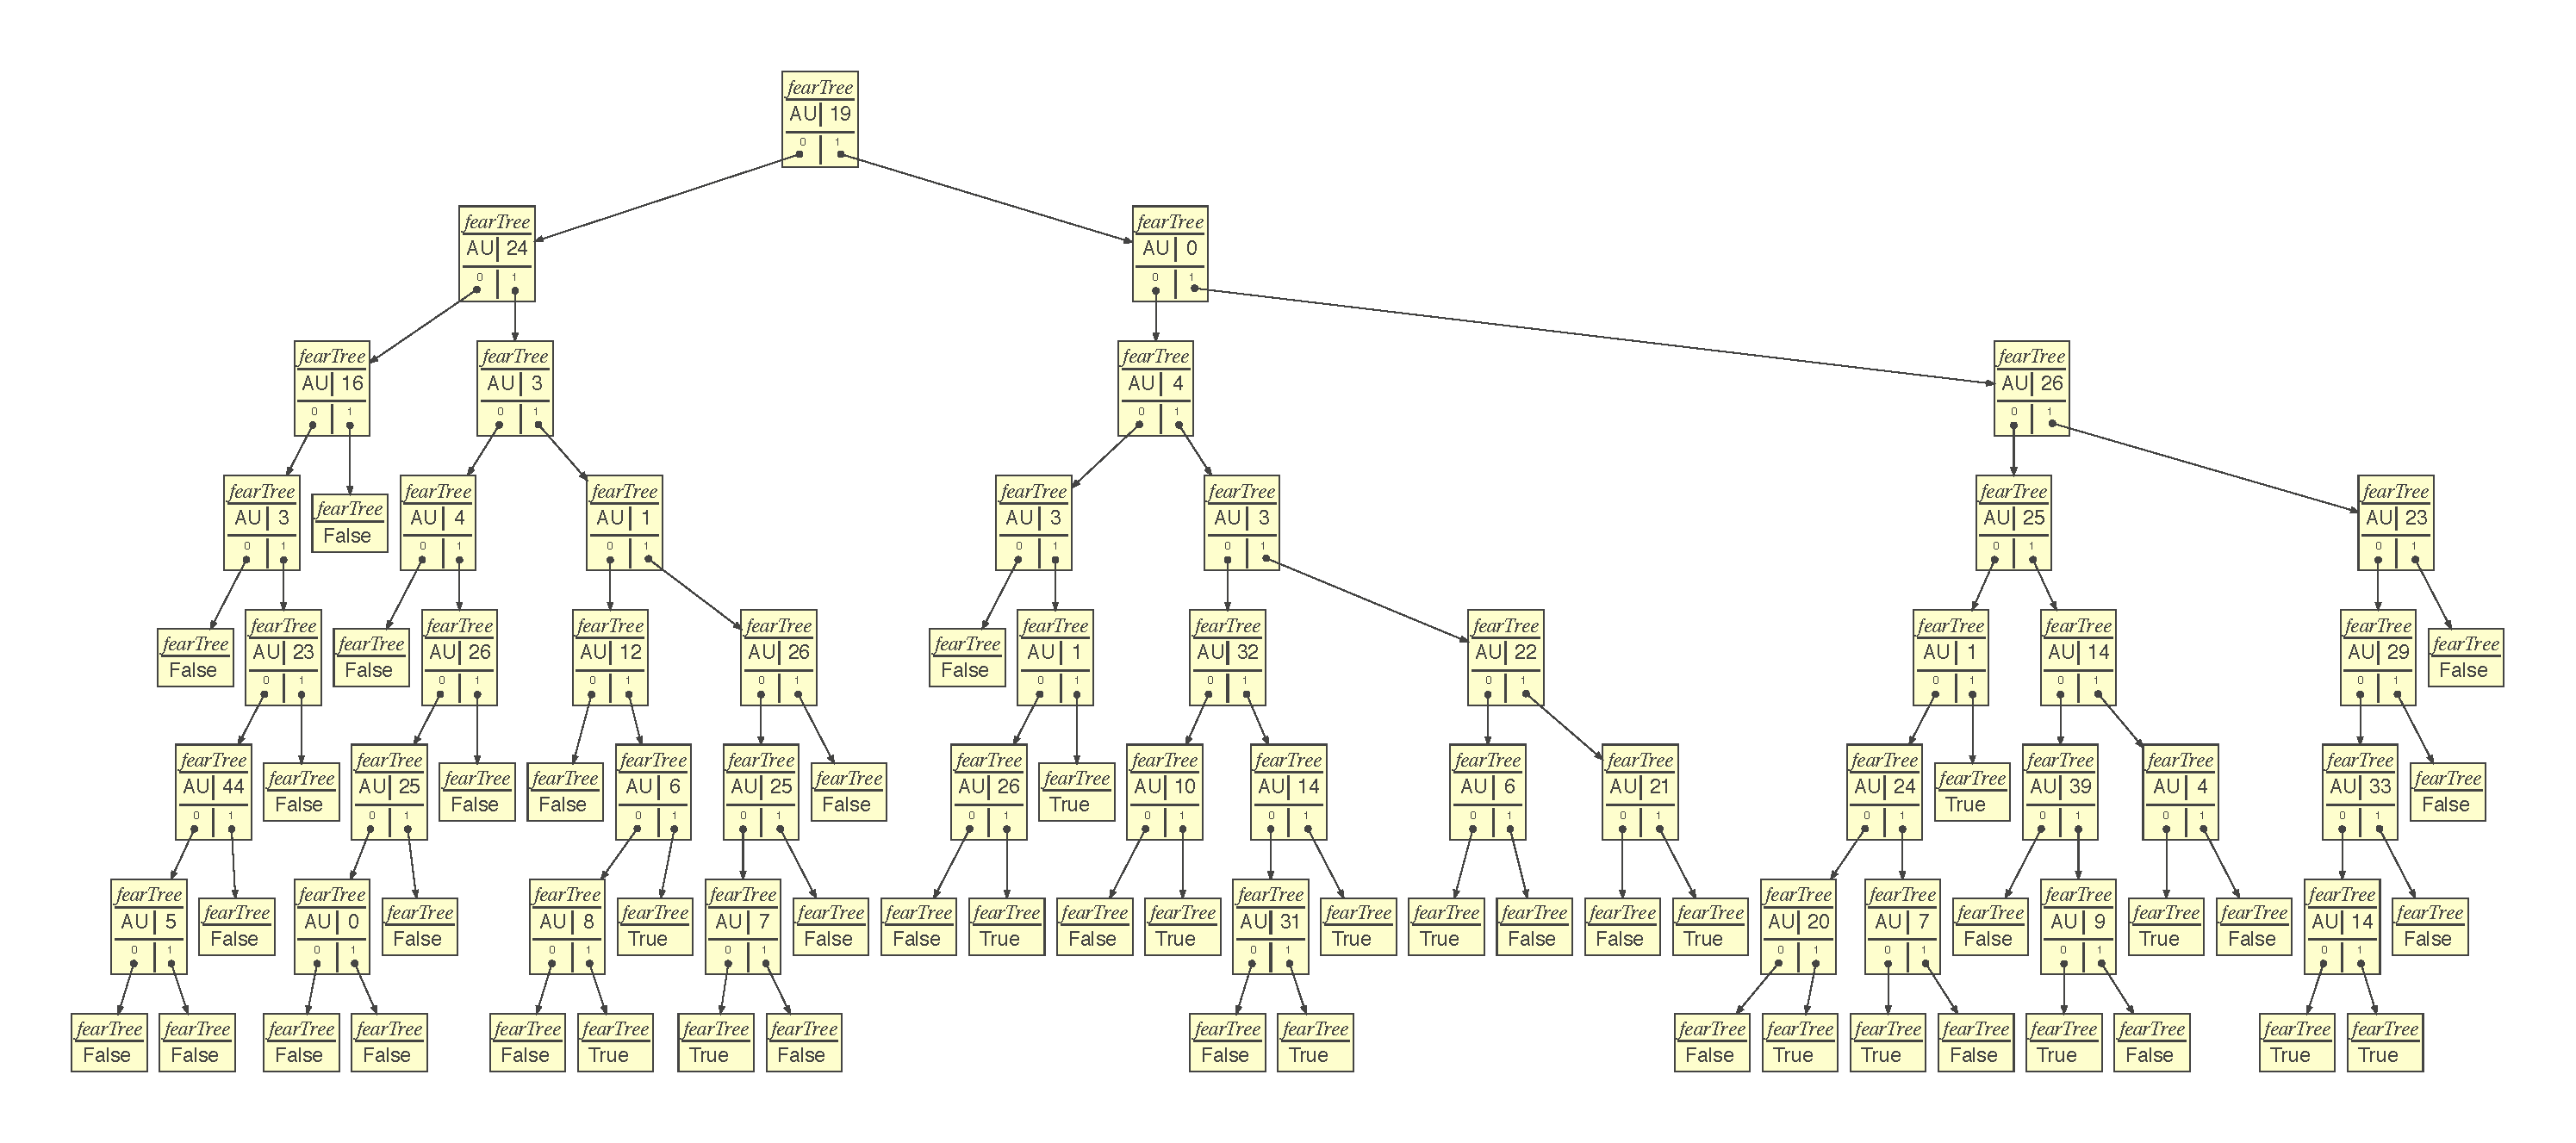
\includegraphics[width=\textwidth]{treePics/fearTree.pdf}
\caption{Fear Tree}
\end{figure}
\begin{figure}[!hb]
\centering
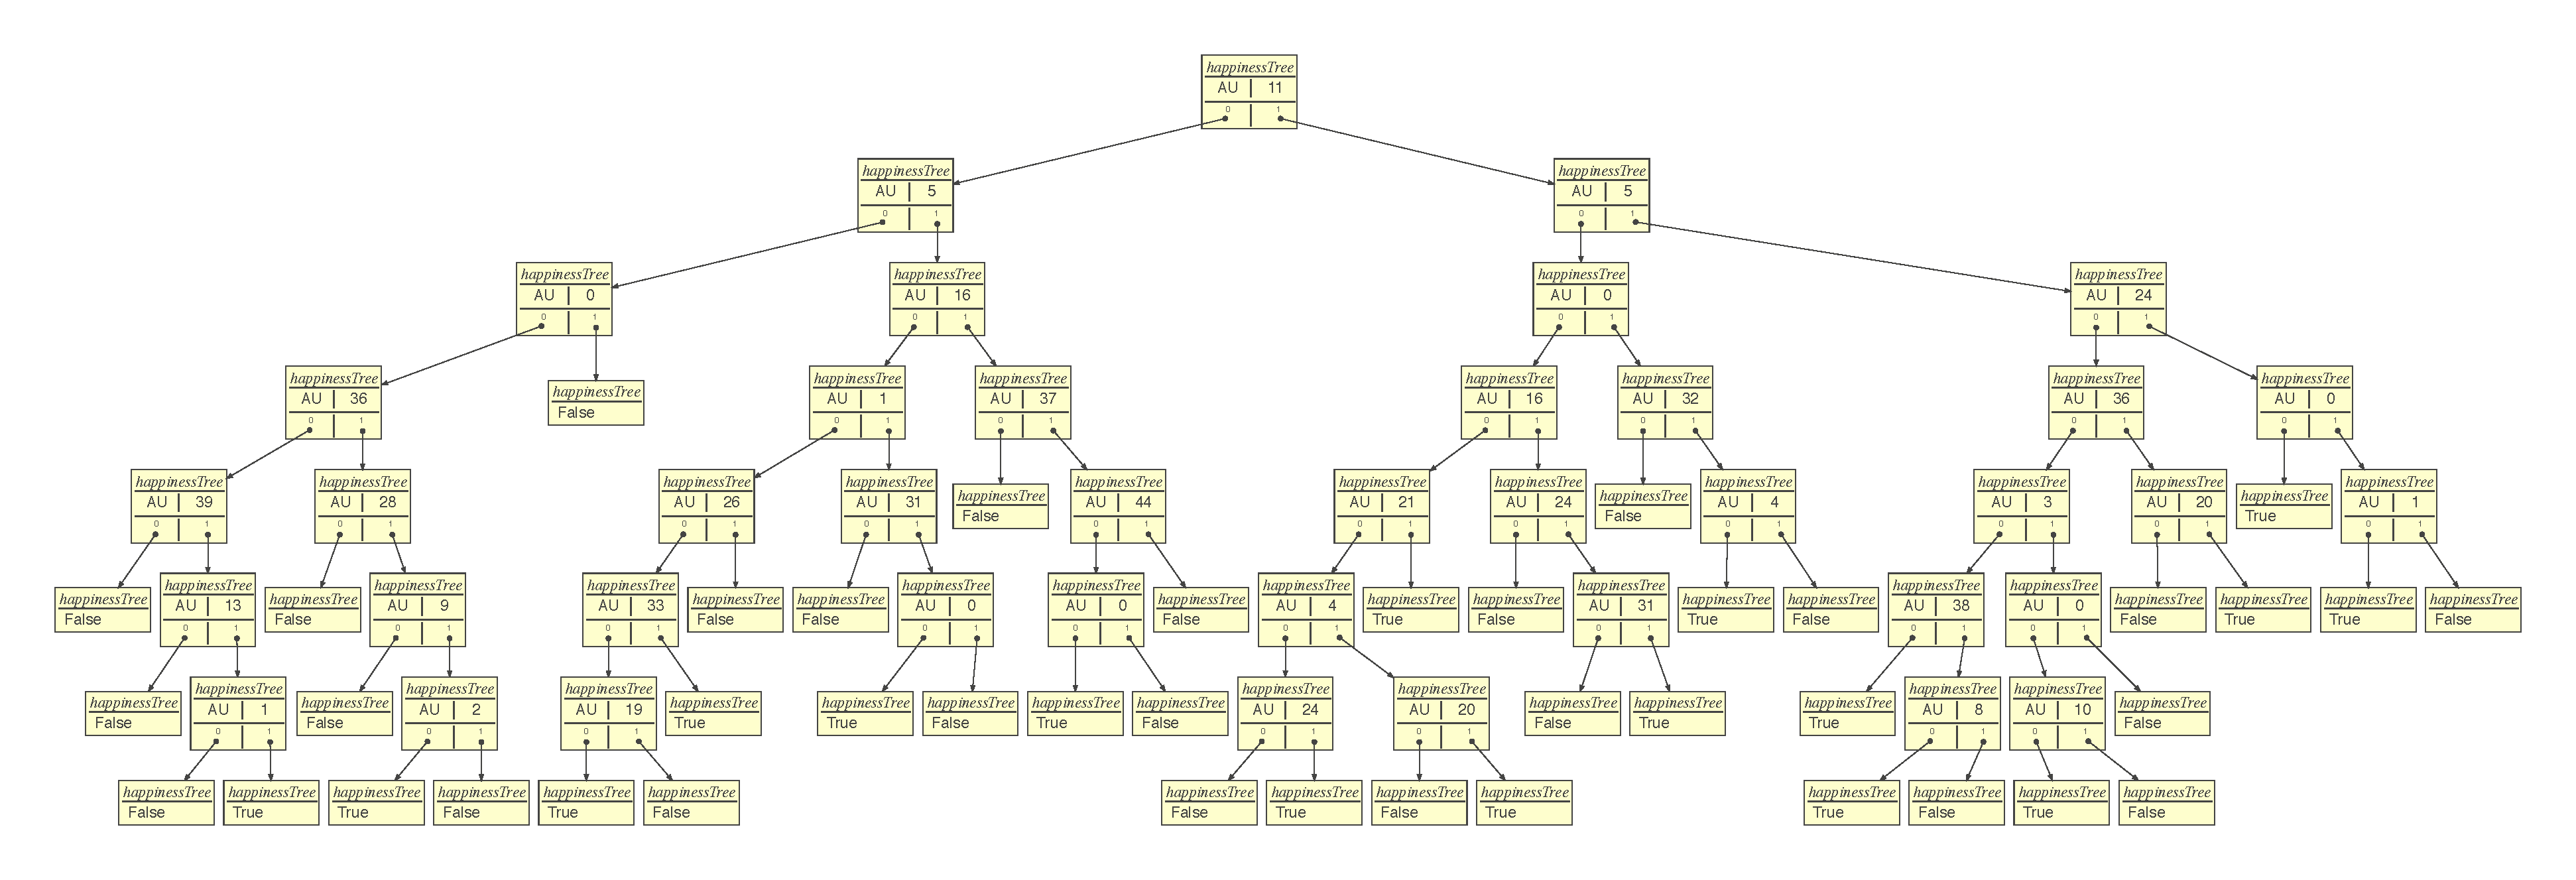
\includegraphics[width=\textwidth]{treePics/happinessTree.pdf}
\caption{Happiness Tree}
\end{figure}
\begin{figure}[!hb]
\centering
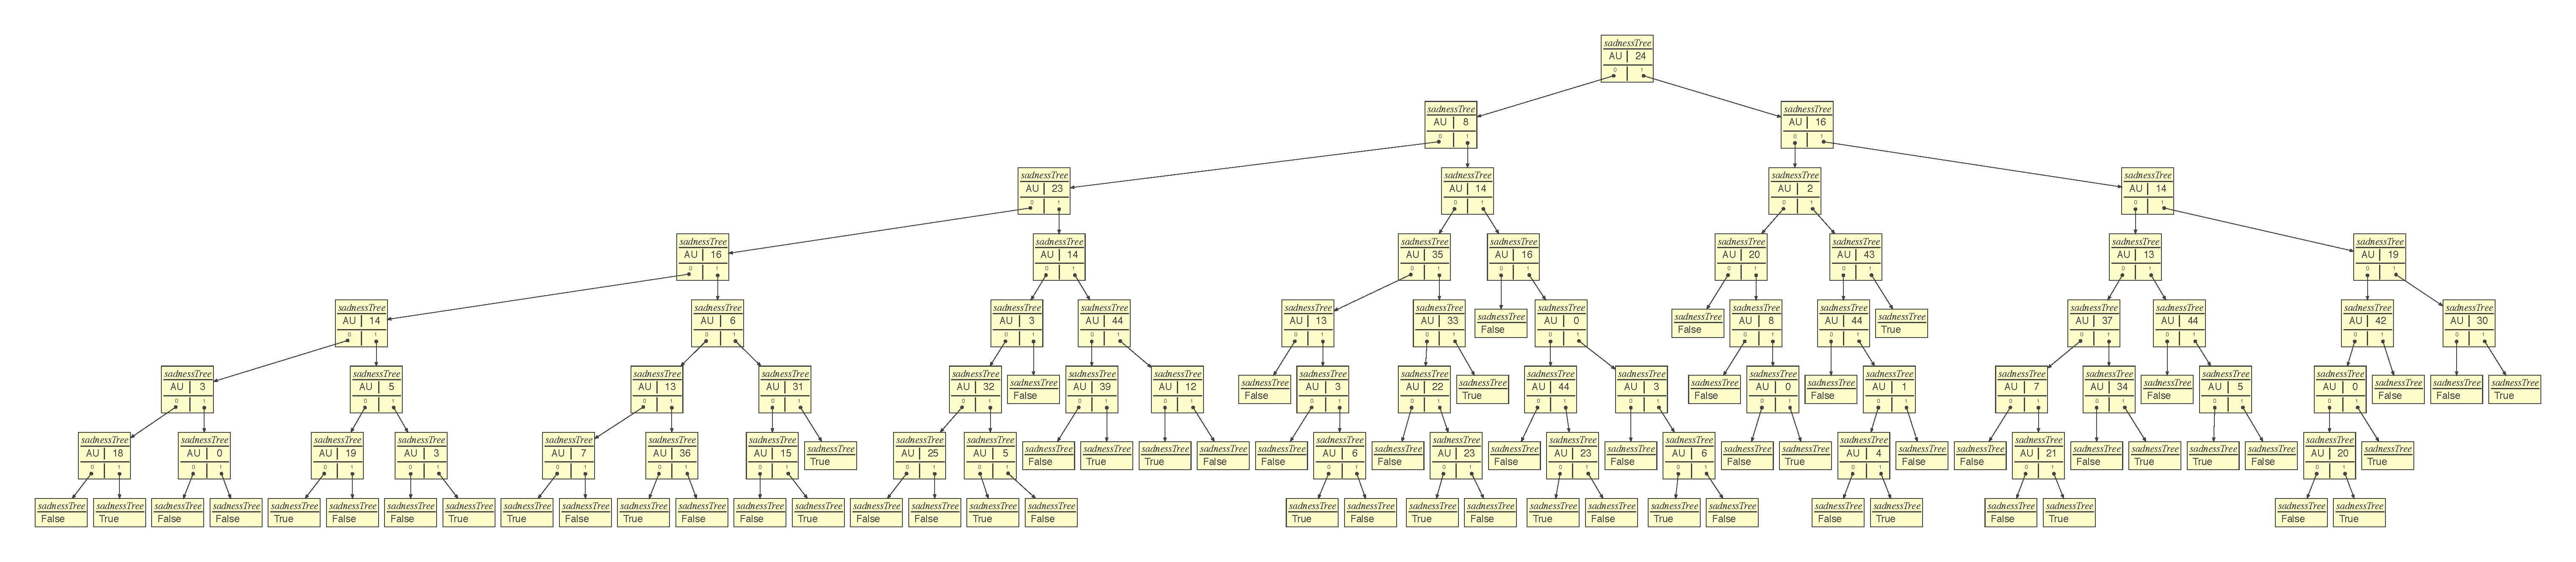
\includegraphics[width=\textwidth]{treePics/sadnessTree.pdf}
\caption{Sadness Tree}
\end{figure}
\begin{figure}[!hb]
\centering
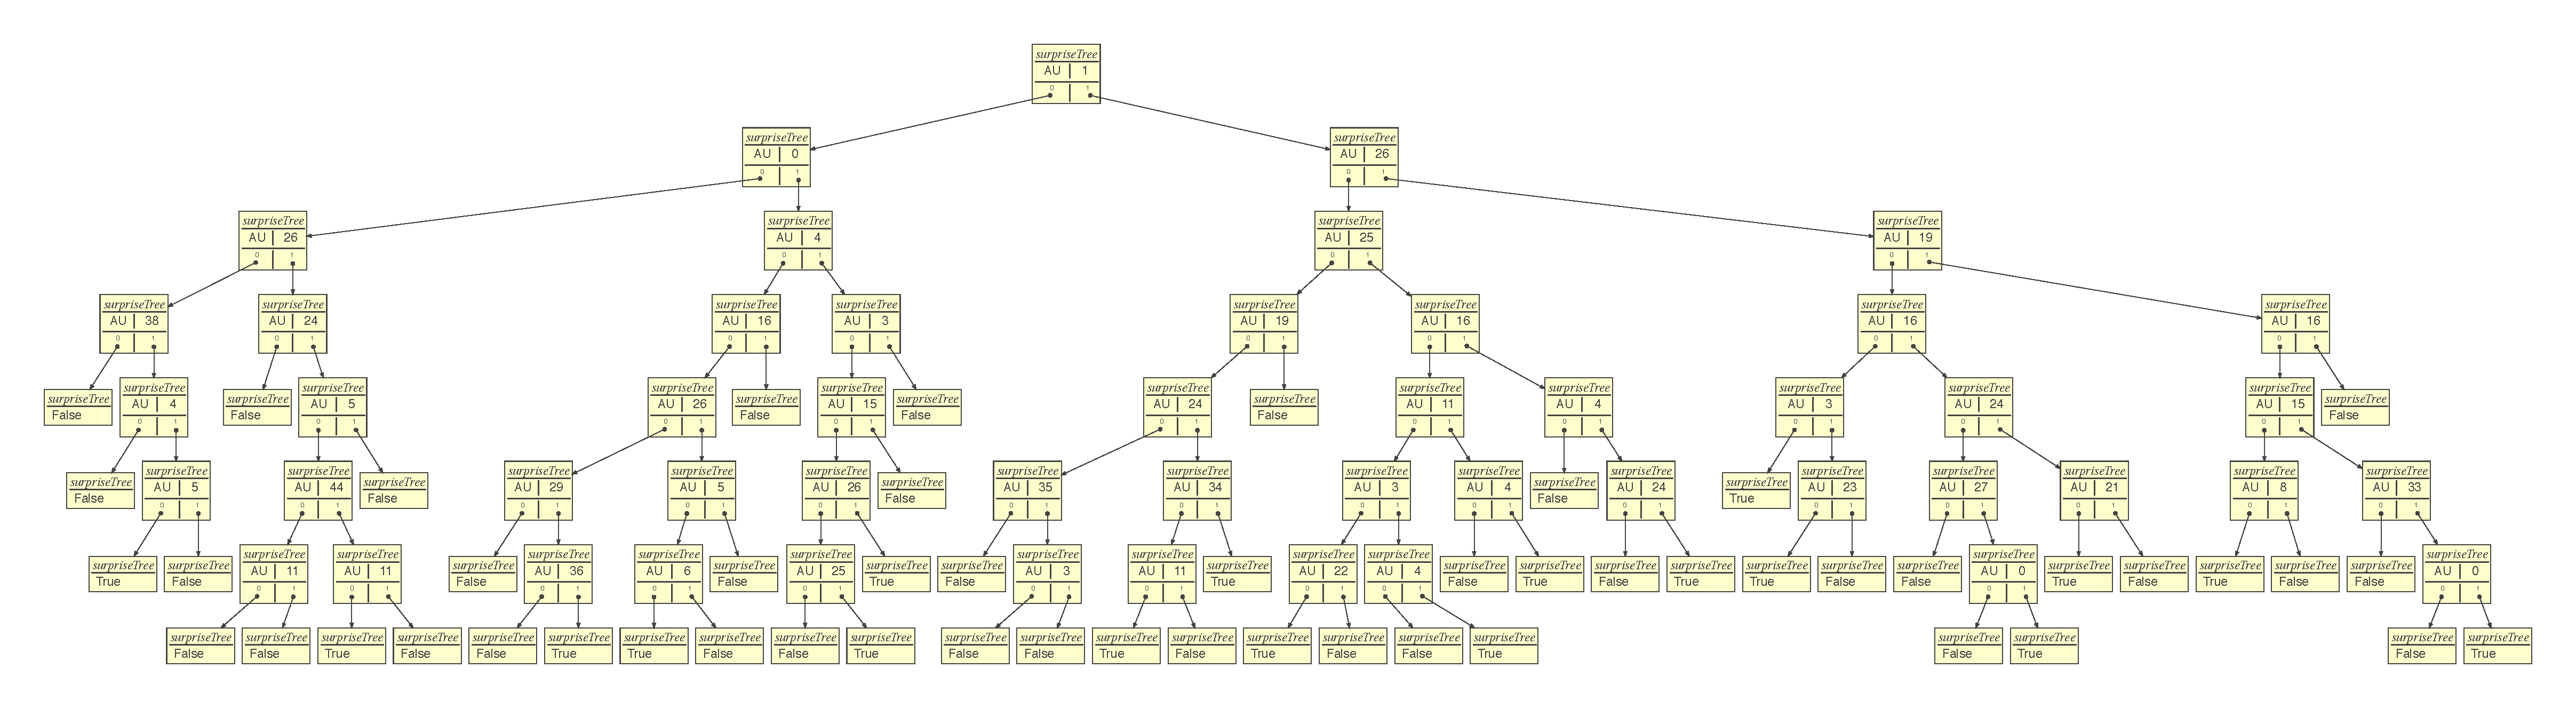
\includegraphics[width=\textwidth]{treePics/surpriseTree.pdf}
\caption{Surprise Tree}
\label{lastTree}
\end{figure}
\end{document}
